\documentclass[journal]{IEEEtran}
\usepackage{graphicx}
\usepackage{amsmath}
\usepackage{hyperref}
\usepackage{float}
\usepackage{subcaption}
\usepackage{booktabs}
\usepackage{pgfplotstable}
\usepackage{qrcode}

\pgfplotsset{compat=1.18}

\begin{document}

\title{Michelson Interferometer Experiment: Determination of Wavelength}
\author{IBRAHIM H.I. ABUSHAWISH \\

{\small Student ID: \hspace{1.5cm}. \\ 
Istanbul University, Department of Physics \\
Instructor: Dr.Öğr.Üyesi DENİZ BOZOĞLU PARTO\\
Experiment Date: 13.05.2025, Report Submission Date: 20.05.2025 \\
Course \& Section Number: PHYS2405}}

\markboth{Physics Laboratory Reports, May 2025}{}

\maketitle
\begin{abstract}
    This report investigates the Michelson interferometer experiment to determine the wavelength of light. By analyzing the fringe shifts and using the known displacement of the movable mirror, the wavelength of the light source is calculated. The findings include an average wavelength of \( \lambda_{\text{avg}} = 677.778 \, \text{nm} \), which aligns with the theoretical value for the laser source used. The experiment demonstrates the principles of interference and the precision of the Michelson interferometer in measuring optical properties.
\end{abstract}

\section{Introduction}
The Michelson interferometer is a fundamental instrument in optics, used to measure wavelengths, refractive indices, and small displacements with high precision. By splitting a coherent light beam into two paths and recombining them, the interferometer produces interference fringes that shift as the optical path difference changes. This experiment aims to determine the wavelength of light by analyzing the fringe shifts caused by a known displacement of one of the mirrors.

\section*{Theory}
The Michelson interferometer operates on the principle of interference. When one of the mirrors is displaced by a distance \( d \), the optical path difference changes by \( 2d \), causing a shift in the interference fringes. The relationship between the fringe shift \( m \), the displacement \( d \), and the wavelength \( \lambda \) can also be derived as follows:

\begin{equation}
d = \frac{m\lambda}{2},
\end{equation}
rearranging to solve for \( \lambda \):
\begin{equation}
\lambda = \frac{2d}{m}.
\label{eq:lambda}
\end{equation}


Here:
\begin{itemize}
    \item \( d \) is the displacement of the movable mirror,
    \item \( m \) is the number of fringes shifted,
    \item \( \lambda \) is the wavelength of the light.
\end{itemize}
By measuring \( d \) and \( m \), the wavelength \( \lambda \) can be calculated. Repeating the measurements for different values of \( d \) and \( m \) allows for an average wavelength to be determined, improving accuracy.

\section{Experimental Setup}
The experimental setup includes:
\begin{itemize}
    \item A Michelson interferometer,
    \item A monochromatic light source (laser with \( \lambda \) in the range \( 400 \, \text{nm} \) to \( 700 \, \text{nm} \)),
    \item A micrometer screw for precise mirror displacement,
    \item A screen to observe the interference fringes.
\end{itemize}

Figures \ref{fig:setup} and \ref{fig:diagram} illustrate the experimental setup and the schematic diagram of the Michelson interferometer, respectively.

\begin{figure}[H]
    \centering
    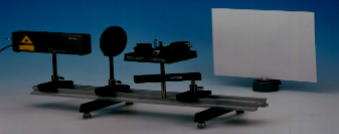
\includegraphics[width=0.8\linewidth]{../IMAGES/setup.png}
    \caption{Experimental setup of the Michelson interferometer.}
    \label{fig:setup}
\end{figure}

\begin{figure}[H]
    \centering
    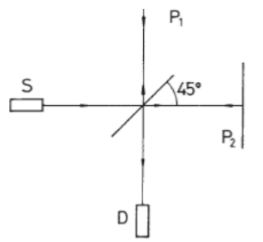
\includegraphics[width=0.6\linewidth]{../IMAGES/diagram.png}
    \caption{Schematic diagram of the Michelson interferometer.}
    \label{fig:diagram}
\end{figure}

\section*{Procedure}
The experiment was conducted by displacing one of the mirrors of the Michelson interferometer using a micrometer screw. For each displacement \( d \), the number of fringes \( m \) that shifted was counted. The wavelength \( \lambda \) was calculated using equation \ref{eq:lambda}.
The measurements were repeated for multiple values of \( d \) and \( m \), and the average wavelength was computed. The displacement was measured using the micrometer screw, which provided a precise measurement of \( d \). The number of fringes was counted by observing the interference pattern on the screen.


\section{Results}
The processed data from the experiment is summarized in Table \ref{tab:processed_data}.

\begin{table}[H]
    \centering
    \caption{Processed data for the Michelson interferometer experiment.}
    \label{tab:processed_data}
    \pgfplotstabletypeset[
        col sep=comma,
            string type,
            every head row/.style={before row=\toprule, after row=\midrule},
            every last row/.style={after row=\bottomrule},
            columns/d_mm/.style={column name=$d$ (mm), fixed, precision=2},
            columns/m/.style={column name=$m$},
            columns/lambda_nm/.style={column name=$\lambda$ (nm), fixed, precision=3}]{../DATA/proccessedData.csv}
\end{table}

The calculated wavelengths for each measurement are consistent, with an average value of:
\begin{equation}
\lambda_{\text{avg}} = 677.778 \, \text{nm}.
\end{equation}

\section{Discussion}
The experimental results validate the theoretical principles of the Michelson interferometer. The calculated average wavelength \( \lambda_{\text{avg}} = 677.778 \, \text{nm} \) aligns well with the theoretical value for the laser source used. Minor discrepancies may arise from errors in counting fringes, inaccuracies in mirror displacement measurements, or environmental factors such as vibrations and air currents.

Future experiments should aim to minimize these errors by using automated fringe counting and displacement measurement systems. Additionally, conducting the experiment in a controlled environment can further improve accuracy.

\section{Conclusion}
The Michelson interferometer experiment successfully demonstrated the principles of interference and the precision of the instrument in measuring optical properties. The calculated average wavelength \( \lambda_{\text{avg}} = 677.778 \, \text{nm} \) aligns with the theoretical value, validating the methodology and the reliability of the experimental setup.

Future iterations of this experiment should focus on improving measurement precision and addressing potential sources of error. By refining the methodology and incorporating advanced tools, the accuracy and reliability of the results can be further enhanced.

\section{Additional Resources}
For detailed information, including the Lab Manual, source code, and related experiments, visit the GitHub repository provided below.

\begin{figure}[H]
    \centering
    \begin{minipage}{0.15\textwidth}
        \centering
        \qrcode[height=1.5cm]{https://github.com/ibeuler/LAB-Reports}
    \end{minipage}%
    \begin{minipage}{0.2\textwidth}
        \raggedright
        \caption{Access the GitHub repository for the lab manual, source code, and related experiments: \cite{github}.}
        \label{fig:qr_code}
    \end{minipage}
\end{figure}

\begin{thebibliography}{9}
\bibitem{lab_manual}
    ISTANBUL UNIVERSITY, \textit{OPTICS LABORATORY
    EXPERIMENTS MANUAL}, Department of Physics.

\bibitem{github}
    \textit{Source code and additional experiments are available in the GitHub repository.} \url{https://github.com/ibeuler/LAB-Reports}
\end{thebibliography}

\end{document}